\initial{P}lanet Earth is often called the blue planet due to the dominant blue areas visible when viewing Earth from space.
The blue areas are our vast oceans covering more than 70\% \cite{WikiEarth} of the surface.
These oceans contain and support a broad spectrum of life, and are also a great influence on the Earth's climate and weather.
All species on Earth, eukaryotes and procaryotes alike, are dependent on water in order to survive.
A human can only survive for 5 days without water \cite{SurviveWater}, and even extremophiles called xerophiles, dry loving bacteria, need a tiny amount of water in order to function.
In other words, water is essential to life as we know it and therefore extremely interesting. 

\subsection{Chemical properties}
\initial{A} single water molecule consists of three atoms: one oxygen atom and two hydrogen atoms.
The two hydrogen atoms are bonded covalently to the oxygen atom.
Water's overall structure is bent due to two lone electron pairs and their electromagnetic pull.
The lone pairs are not shared between the atoms.
Furthermore, the oxygen atom is much more electronegative than the hydrogen atoms, creating a dipole moment in the molecule.
This means that the oxygen will contain a slight, but significant negative charge while the two hydrogen atoms appear as slightly positive.
This creates the basis for the formation of an intricate network of hydrogen bonds as we know that positive and negative charges attract one another.

So what makes water so unique?
First of all, the formation of hydrogen bonds gives water a high evaporation entalphy and therefore a large evaporation temperature.
To transform water from its liquid phase to vapor, energy must be applied bringing water to a temperature of 100\degree C.
On the other end of the scale, water will freeze at 0\degree C transforming to ice, which brings us to the second uniqueness of water.
In most cases, a solid phase will be denser than a liquid phase.
Thus the solid phase would sink to the bottom of the liquid phase. \cite{SolidWater}.
Polar bears floating on ice flakes in the Arctic are evidence that ice is not heavier than water.
This phenomenon has had a greater importance than just serving as a fleet for polar bears.
Without this property, ice would have sunk to the bottom in repeated cycles until there was no more liquid water during the cold periods in the history of Earth.
To sum up, due to chemical and physical properties, water remains liquid over a uniquely broad range of temperature.

However, the temperature is not the only thing that decides phase states in matter.
Pressure is equally important.
Therefore one can boil water at 70\degree C at the top Mount Everest (making it hard to boil an egg), while you need to heat it to 100\degree C at sea level \cite{WaterEverest}.
A phase diagram shows how this relationship between temperature and pressure affects the states of water.

\begin{center}
	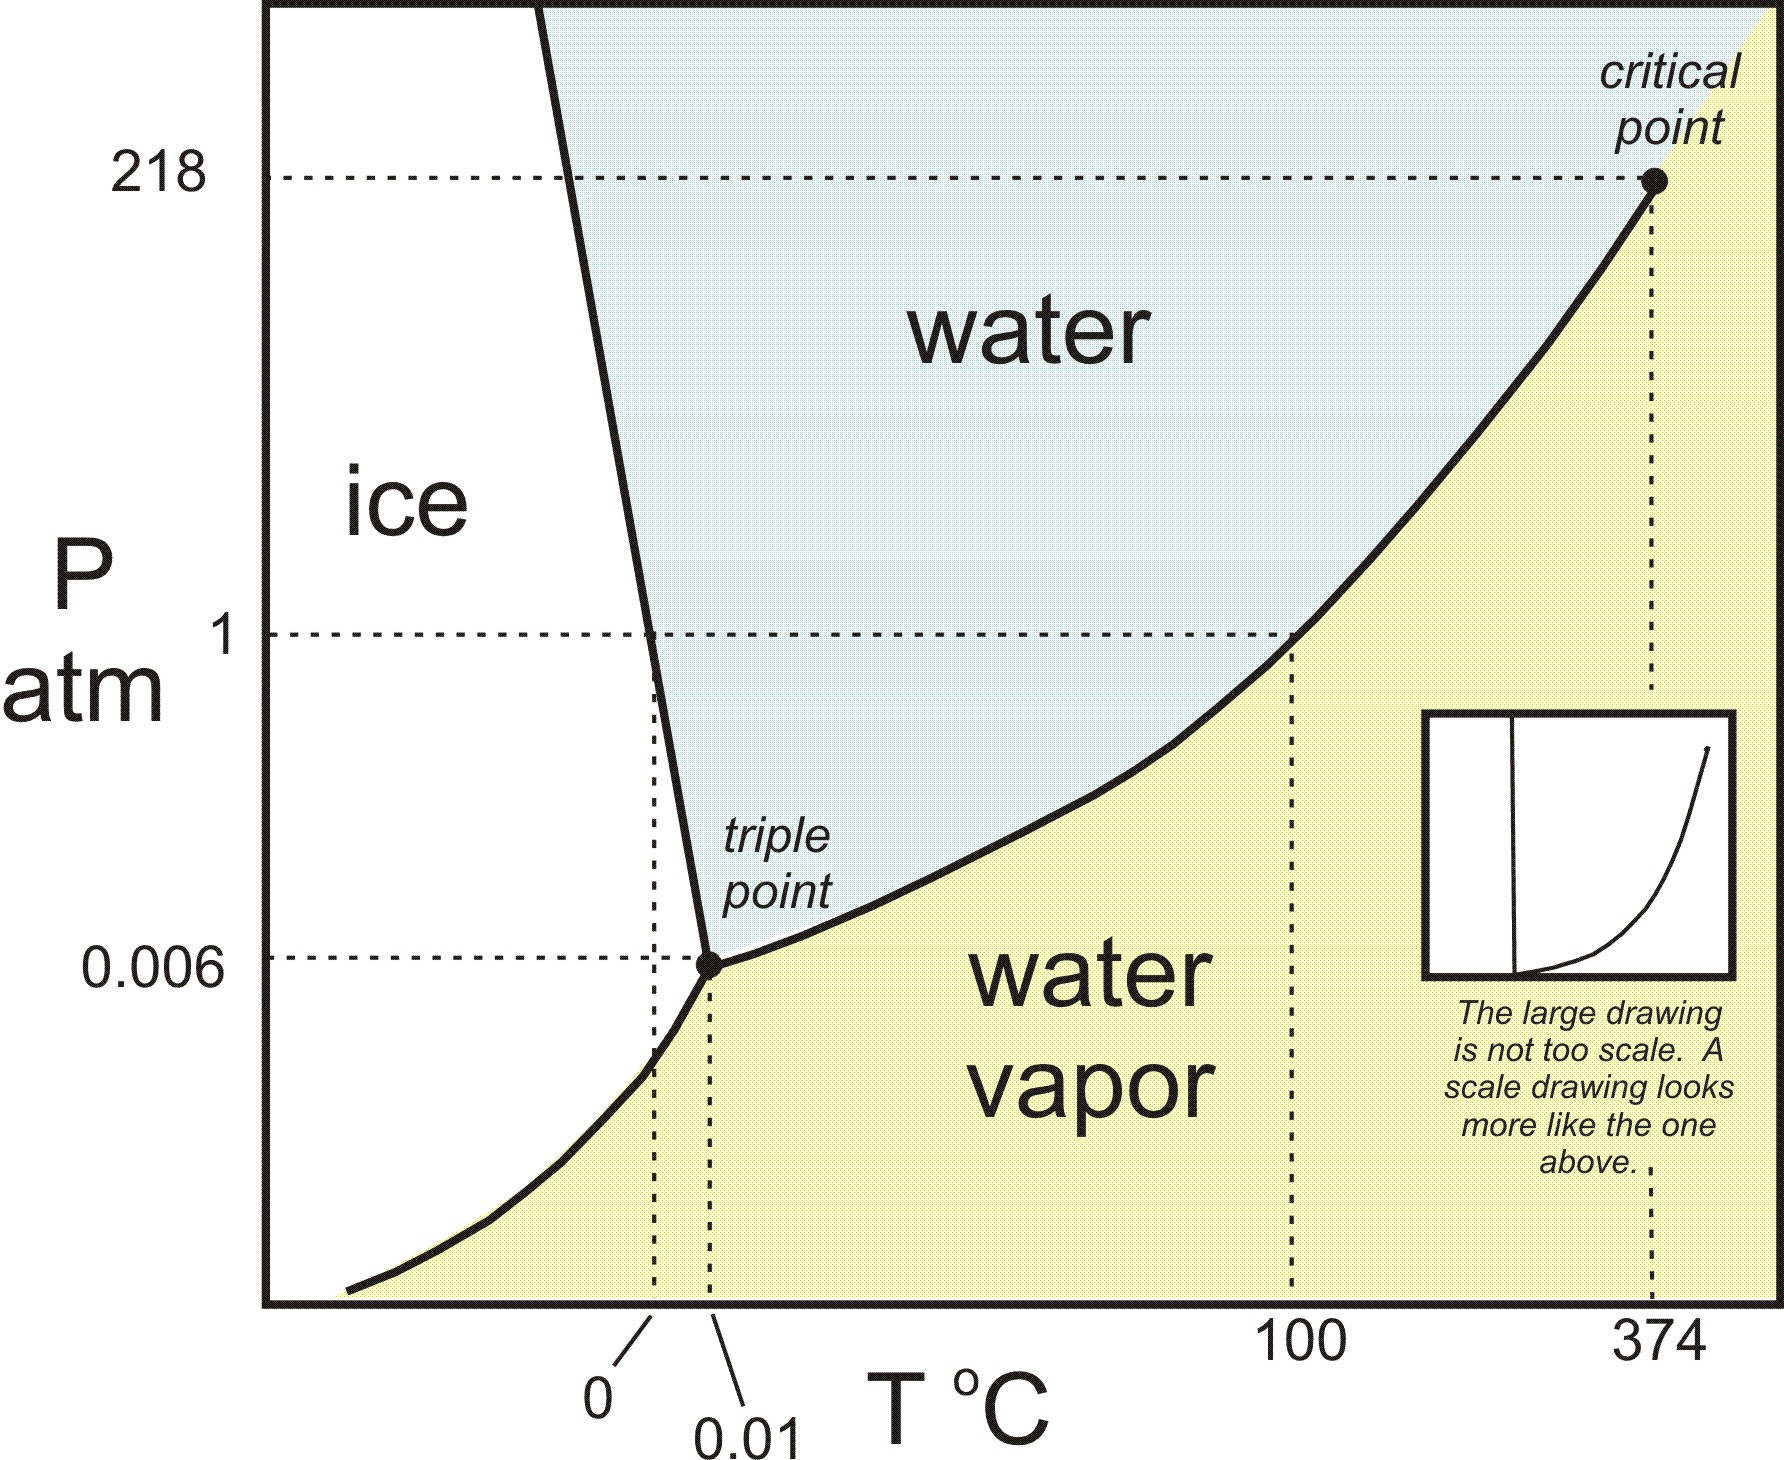
\includegraphics[width=0.475\textwidth]{h2o_phase_diagram.jpg}
	\tiny{Credit: David Mogk, Montana State University}
\end{center}

Although water can appear at Earth's 1 atm, the pressure of 0,006 atm at the Martian surface \cite{NASA-rover} does not allow water to be liquid.
Coincidence makes it so that the pressure on Mars coincides with the triple point of water.
An attempt to melt ice on Mars will result in sublimation, going directly from ice to vapor.
The mean temperature on Earth is 15\degree C \cite{TempEarth}.
This along with the pressure of 1 atm it makes Earth a perfect place for liquid water. 
So far, we have established that we have a lot of water on Earth, and it occurs mostly in its liquid form.
The question remaining is: what is so important with liquid water?

Liquid water has functions as both a solvent and a transport medium.
Both organic and inorganic compounds can be dissolved in water, making it a vital part of metabolism.
The blood stream is an essential transport network delivering oxygen and nutrients in our body.
Human blood plasma, the liquid part of the blood, consists of 92\% water \cite{Blood}.
On Earth, we have yet to find an organism completely independent of water. 
In fact, in all three theories concerning the origin of life, water was given a leading role as a solution bringing the organic molecules together.
As we want to find life, it seems appropriate to base our search on water.
NASAs guiding policy reflects this: \textit{Follow the water} \cite{NASAwater}. 
Water is not a rare molecule in space, in fact oxygen and hydrogen are some of the most abundant atoms in the Universe.
One problem is that the water in space most often is in the solid form of ice, and in rare occasions in form of gas.
Another problem is that space is big, really big!
Bumping into a pool of water by accident is not something that is going to happen any time soon.
Fortunately we have a neighbour that is not too far away.
Mars was first visited decades ago, and as of now there have been several missions to this barren planet.
The rover roaming the surface of the Red Planet today, named Curiosity, does so seeking for evidence of water.